\begin{frame}[allowframebreaks]{Style GANs}
\begin{itemize}
    \item Goal: Better disentanglement of features in latent space (\textbf{W} space)
\end{itemize}
    \begin{figure}
    \centering
    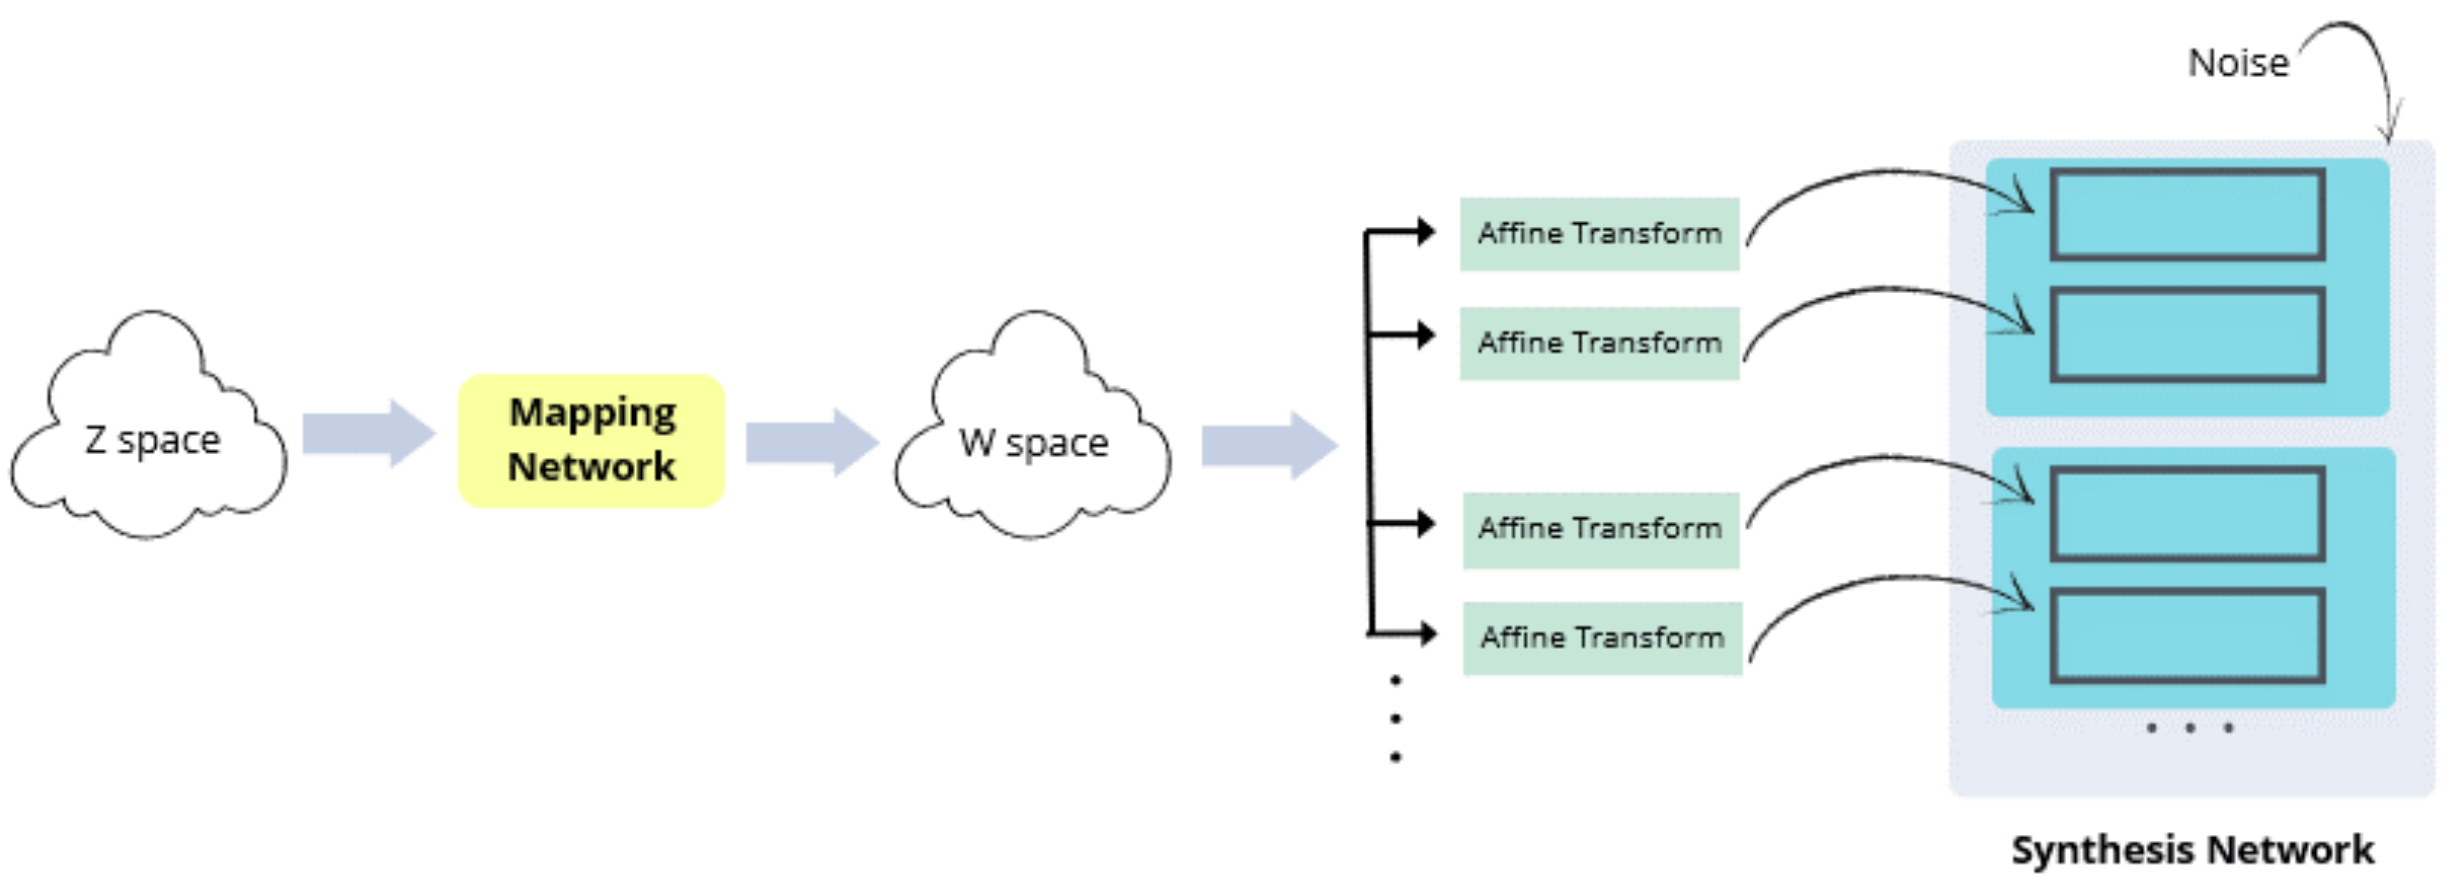
\includegraphics[height=0.9\textheight, width=\textwidth, keepaspectratio]{images/gan/stylegan_2.png}
\end{figure}

\footnotetext{https://www.cs.unc.edu/~ronisen/teaching/fall_2022/pdf_lectures/lecture6_gan2.pdf}
\end{frame}
\begin{frame}[allowframebreaks]{Style GANs}
\begin{figure}
    \centering
    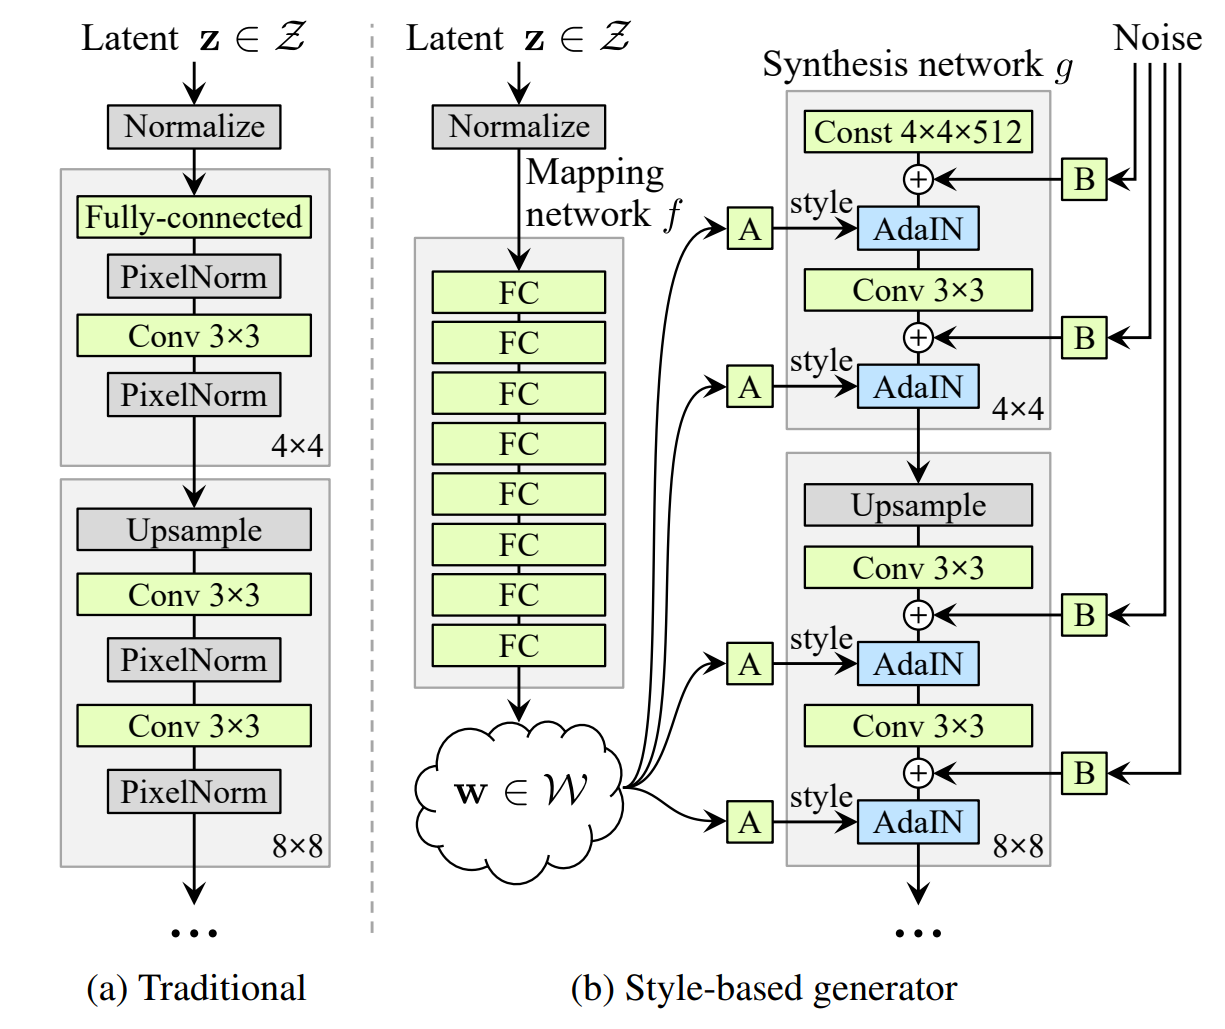
\includegraphics[height=0.9\textheight, width=\textwidth, keepaspectratio]{images/gan/stylegan_1.png}
\end{figure}
\footnotetext{https://arxiv.org/pdf/1812.04948}
\end{frame}
\begin{frame}[allowframebreaks]{Style GANs}

\begin{itemize}
    \item \textbf{A} = learned affine transformation block for AdaIN (predicts y)
    \item \textbf{Ada}ptive \textbf{I}stance \textbf{N}ormalization (very effective in controlling styles)
    $$\text{AdaIN}(x_i,y) = y_{s,i}\frac{x_i - u(x_i}{\sigma(x_i)} + y_{b,i}$$
    \item \textbf{B} = learned per-channel scaling factor for noise input.

\end{itemize}

\end{frame}

\begin{frame}[allowframebreaks]{Which Latent space to choose for embedding and editing?}
\begin{itemize}
    \item \textbf{Z} : 512 dimensional latent space (not good)
    \item \textbf{W} : 512 dimensional latent space (better but not perfect)
    \item \textbf{W+} : 18x512 dimensional latent space (after affine transformation \textbf{A} has been applied)
    \item \textbf{W} is better for editing.
    \item \textbf{W+} is better for reconstruction or embedding of real images.
\end{itemize}

\end{frame}

\begin{frame}[allowframebreaks]{Style GANs - Results}
\begin{figure}
    \centering
    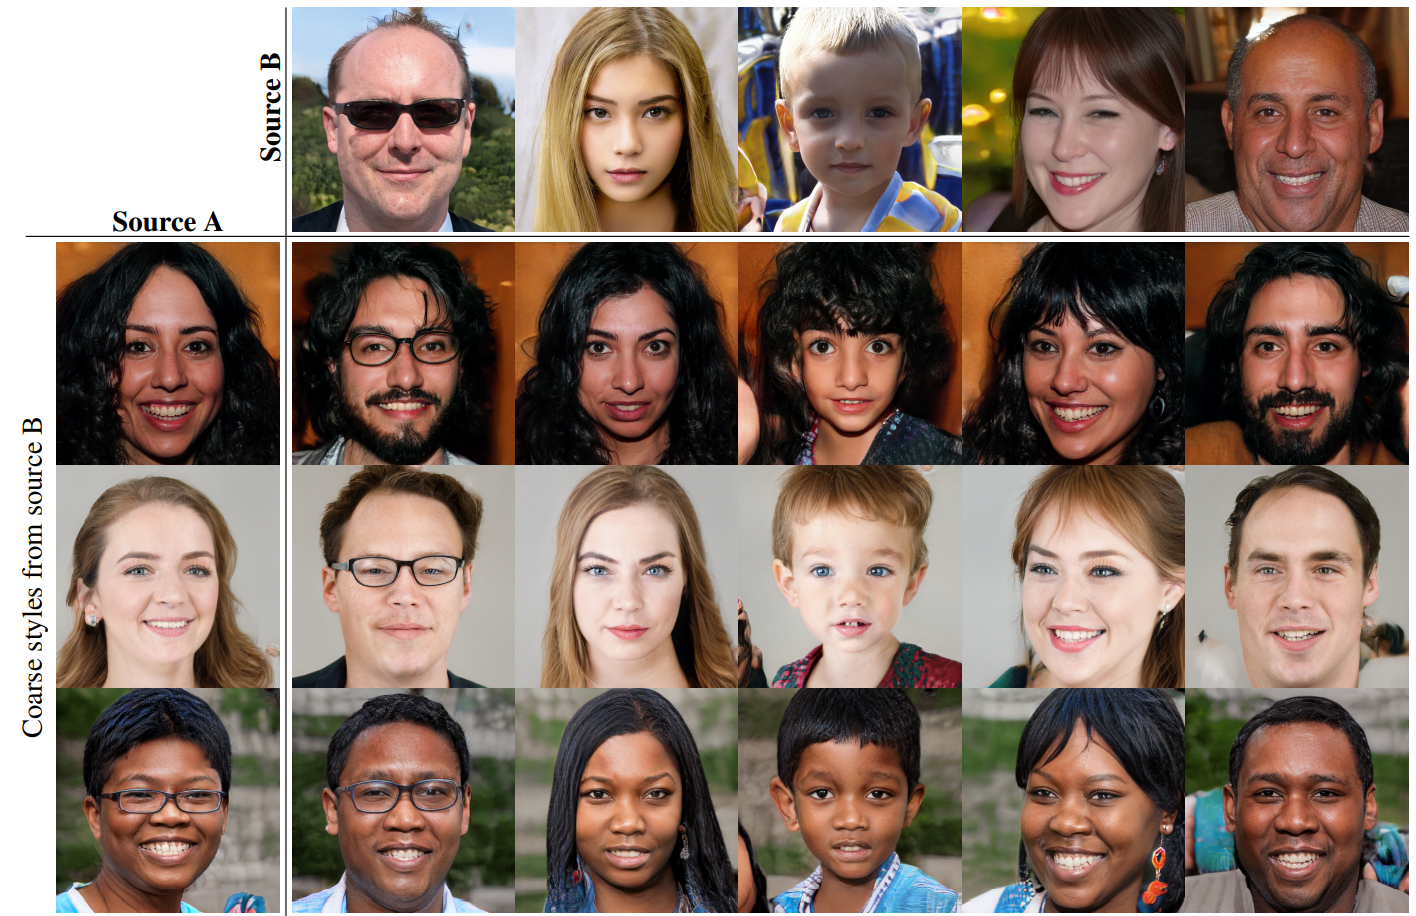
\includegraphics[height=0.9\textheight, width=\textwidth, keepaspectratio]{images/gan/stylegan_3.png}
\end{figure}
\footnotetext{https://arxiv.org/pdf/1812.04948}
\end{frame}